\documentclass[11pt]{article}

%%%%%%%%%%%%%%%%%%%%%%%%%%%%%%%%%%%%%%%%%%%%%%%%%%%%%%%%%%%%%%%%%%%%%%%%%
\pagestyle{plain}                                                      %%
%%%%%%%%%% EXACT 1in MARGINS %%%%%%%                                   %%
\setlength{\textwidth}{6.5in}     %%                                   %%
\setlength{\oddsidemargin}{0in}   %% (It is recommended that you       %%
\setlength{\evensidemargin}{0in}  %%  not change these parameters,     %%
\setlength{\textheight}{8.5in}    %%  at the risk of having your       %%
\setlength{\topmargin}{0in}       %%  proposal dismissed on the basis  %%
\setlength{\headheight}{0in}      %%  of incorrect formatting!!!)      %%
\setlength{\headsep}{0in}         %%                                   %%
\setlength{\footskip}{0in}       %%                                   %%
%%%%%%%%%%%%%%%%%%%%%%%%%%%%%%%%%%%%                                   %%
\newcommand{\required}[1]{\section*{\hfil #1\hfil}}                    %%
\renewcommand{\refname}{\hfil References Cited\hfil}                                      %%
%%%%%%%%%%%%%%%%%%%%%%%%%%%%%%%%%%%%%%%%%%%%%%%%%%%%%%%%%%%%%%%%%%%%%%%%%

%PUT YOUR MACROS HERE
\usepackage[backend=biber,style=authoryear,sorting=none]{biblatex}
\addbibresource{phd_bombus.bib}
\usepackage{amsmath}
\usepackage{amssymb}
\usepackage{sectsty}
\usepackage{hyperref}
\usepackage{graphicx}
\usepackage{float}
\usepackage{textcomp}
\sectionfont{\normalsize\bfseries}

\pagestyle{empty}



\begin{document}
\setcounter{page}{1}
\begin{center}
\textbf{Spatially-explicit mark-recapture models for inferring bumblebee foraging range}

Jenna Melanson
\end{center}

\noindent \textbf{Abstract}

 For central-place foragers like bumblebees, the spatial distribution of resources in the vicinity of established nest sites plays a key role in determining reproductive success. Foragers can maximize their rate of energy returns by visiting resource patches which are closer to the nest or contain a higher quantity of floral rewards. In intensively managed agroecosystems, where flowers are patchily distributed and may appear in transient pulses (e.g., mass-flowering crops) species with greater behavioural plasticity or the ability to visit distant, high-quality patches may be more successful. Using a spatial mark-recapture dataset, I investigate the difference in foraging scales for two bumblebee species: a widespread native species and a rapidly expanding invasive known to prefer anthropogenically disturbed habitats. I first show that mark-recapture data carry more information regarding \emph{relative} foraging distance than \emph{absolute} foraging distance, and describe different strategies for preventing overestimation of foraging range in high-dimensional parameter space; using my best model, I show that invasive \emph{Bombus impatiens} forages at a greater scale than native \emph{Bombus mixtus}. Next, I expand to the model to incorporate the impacts of local and landscape-scale resource availability on relative foraging range. I perform simulations across a range of data-generating values to show that local-scale resource effects are easier to detect than landscape-scale resource effects when using biologically/experimentally realistic data. The analyses provide insight regarding the importance of informative priors in high-dimensional models, and result in a (relatively) robust pathway for estimating resource effects on bumblebee foraging scale.


\noindent \textbf{Introduction}

Global food security is highly dependent on the conservation of animal pollinators in landscapes managed for food production \parencite{kremen_crop_2002, eilers_contribution_2011}. Agricultural intensification is a multi-facted process which involves expansion of monoculture crop systems, reduction of non-crop habitat, and removal or replacement of native vegetation \parencite{emmerson_chapter_2016}, resulting in reduced or altered patterns of resource availability for pollinators. Theoretical models have suggested that species-level variation in traits linked to foraging scale and patch attractiveness may disproportionately favour some ``winner" species in structurally simple landscapes \parencite{bolin_scaledependent_2018}; therefore, to more effectively preserve pollinators in agricultural landscapes, it is important to understand how changes in resource availability across spatial scales influences foraging patterns, and how these trends differ between species.
 
One method for assessing foraging scale and colony density of social bees is through the use of genetic mark-recapture datasets. Each colony is a unit which can be ``recaptured" through repeated observations of genetically-similar sibling colonymates \parencite{chapman_genetic_2003}. By collecting such observations across a spatially-explicit trapping grid, it is possible to produce estimates of ``minimum maximum" foraging distance and to regress pairwise sibling-separation distances against covariates of interest (e.g., \textcite{jha_resource_2013}). The latter method implicitly assumes continuous spatial sampling, and can produce spurious correlations for discrete trapping datasets \parencite{pope_inferring_2017}. More recently, spatially explicit frameworks have been used to model discrete trapping data \parencite{pope_seasonal_2018}.

Here, I build upon previous models to investigate differences in foraging scale and its dependence on local and landscape-scale resource availability for two bumblebee species (\emph{Bombus mixtus} and \emph{B. impatiens}).
 
\noindent \textbf{Methods}

To make estimates of colony foraging range, I modelled visitation of colony $i$ at trap $k$ as a function of the distance between trap location $z_k$ and the latent colony location $\delta_i$. I compute the multinomial probabilities of a visitor from colony $i$ occurring at each trap $k \in K_L$ where I surveyed for the colony, and condition the model on the observed counts of workers from each colony at each trap. Below I give the joint distribution, where $\mathbf{y}_i$ is the vector of counts for colony $i$, $\rho$ denotes the length scale of foraging, and $\epsilon_k$ are trap-specific intercepts.

\[
\mathbf{y}_i \sim \text{Multinomial}\big(n_i, \mathbf{p}_i \big)
\]
\[
p_{ik} = \frac{\lambda_{ik}}{\sum_{j=1}^{K_l} \lambda_{ij}}, 
    n_i = \sum_{j=1}^{K_l} y_{ij}
\]
\[
log(\lambda_{ik}) = -\frac{1}{2}\left(\frac{\lVert z_k - \delta_i \rVert}{\rho}\right)^2 + \epsilon_k
\]

\noindent I specify priors $\rho \sim lognormal(log(0.5), 0.5)$, $\epsilon \sim \mathbb{N}(0, \sigma^2)$, and $\sigma \sim exponential(1)$.  Unless otherwise specified, $\delta$ receives an implicit uniform prior; to speed up computation, I limit the bounds on this prior to $\pm 5$km easting/northing from the trapping grid where the colony was observed. I conduct model inference using Stan \parencite{carpenter_stan_2017} implemented via \emph{rstan} \parencite{rstan}. 

I collected bumblebee colonymates across six replicate landscapes in the Lower Fraser Valley (BC, Canada) during the spring/summer of 2022 \& 2023 (see Appendix section "Data Collection" for details). I simulated data in \emph{R} version 4.4.3 \parencite{r_core_team_r_2021} following \textcite{pope_inferring_2017} (see Appendix section "Simulating Data" for details). When not otherwise mentioned, data were simulated to closely replicate real data: i.e., similar sample size (number of bees), siblingship size distribution (number of bees per colony observed), and identical trapping configuration. The empirical data are currently unpublished, but code for simulation and modelling can be found at \url{https://github.com/jmelanson98/stat547/tree/main/final_project}. \\

\noindent \textbf{Section 1: How accurately can we estimate absolute foraging distance?}

I first conditioned the simple model above on three datasets: (1) an ``ideal" simulated dataset, consisting of 531 colonies with an average siblingship size of 37 (Fig \ref{fig:fig1}A), (2) a biologically realistic simulated dataset, consisting of 1438 colonies with an average siblingship size of 1.4 (Fig \ref{fig:fig1}B), and (3) data collected in the field for \emph{B. impatiens}, consisting of 2632 colonies with average siblingship size of 1.3 (Fig \ref{fig:fig1}C). Both simulated datasets were produced with a data-generating value of $\rho = 0.5$km (e.g., 95\% of foraging activity occurs within approx. 1km of the nest). 

The inferred posterior means for $\rho$ were 0.90 (95\% credible interval: 0.88-0.92) (ideal simulated dataset), 1.43 (95\% credible interval: 1.35-1.52) (biologically realistic simulated data), and 1.22 (95\% credible interval: 1.16-1.28) (\emph{B. impatiens} dataset) (Fig \ref{fig:fig1}D-F). The discrepancy of both simulated results from the data-generating $\rho = 0.5$ is surprising, particuarly for the (presumably) highly-informative ideal dataset. 

The pairs plots offer us a hint as to what may be occurring --- in all cases, $\rho$ is strongly negatively correlated with the unnormalized log joint posterior density. Indeed, when I fix $\rho$ across a range of values and compute the optimum of the log joint posterior density, I find that the joint density is largest for smaller $\rho$, or in the case of the ideal dataset, for $\rho = 0.5$ (Fig \ref{fig:fig1}G-I). Recall that the support for a model is the product of the likelihood and the area over which the likelihood is integrated --- while the joint density may be maximized for small $\rho$, small values of $\rho$ are restrictive on other terms in the model (e.g., the high-dimensional vector of latent colony locations, $\delta$). This reduces the volume of the parameter space which is consistent with the data. Larger $\rho$ values can achieve greater posterior mass because their lower likelihood is compensated by greater volume in the latent space. This phenomenon is analagous to the typical set in high dimensions, as described in \textcite{betancourt_conceptual_2018}.

Based on the shape of the optimized log joint posterior profiles (Fig \ref{fig:fig1}D-F)) it seems unlikely that we will be able to achieve accurate estimation of absolute foraging distance for a biologically realistic dataset; while all three profiles appear to favour small values of $\rho$, only the ideal dataset is able to pinpoint the data-generating value.\\

\noindent \textbf{Section 2: Constraining $\delta$ to achieve esimates of relative foraging distance}

Devastated by my failure to infer absolute foraging distance with biologically realistic data, I next move to comparisons between species. If the data generating $\rho$ is greater for species A than species B, can we detect this difference?

I start by testing three methods to more strongly inform $\delta$ and reduce the influence of large parameter volume in high dimensions. The first of these methods is to simple remove the trap-specific intercepts $\epsilon_k$ from the model likelihood --- these intercepts may allow greater model flexibility than is desireable, permitting extreme configurations of $\delta$ when $\sigma$ is large.

A second strategy is to restrict colony locations to some radius $R_{max}$. I achieve this by applying either a Gaussian or pseudo-Uniform penalization to the target density when $\delta_i$ is further than $R_{max}$ from the trap(s) where colony $i$ is observed (see \ref{fig:A1} for details on specification). This penalization is not a proper prior, as it incorporates data on where the colony is observed. 

Finally, we can apply a bivariate Gaussian prior on $\delta$ which is centered at the middle of the trapping grid\footnote{This prior should not be interpreted biologically (e.g., ``bumblebees are more likely to nest at the center of trapping grids because they have an affinity for graduate students in high-vis vests") but rather as a prior on the observational process. The colonies we detect are only a subset of all colonies located on the landscape --- indeed, if we fit the distribution of siblingships sizes (Fig \ref{fig:fig1}C) to a truncated Poisson to estimate the zero-class, we find that the majority of colonies are not observed at all. While colonies in general may be uniformly distributed, we are most likely to observe those near the center of the trapping grid, as we have surveyed a larger proportion of their foraging kernel than we have for colonies located on the periphery.}:

\[
\delta =
\begin{pmatrix} \delta_x \\ \delta_y \end{pmatrix}
\sim \mathcal{N}\Big(\boldsymbol{0}, \sigma_d \mathbb{I}\Big)
\]

For each of the methods described above, I again compute the posteriors and profile log posteriors for the ideal simulated dataset (Fig \ref{fig:perfectentropyfix}) and the biologially realistic simulated dataset (Fig \ref{fig:realentropyfix}). For the ideal dataset, we can see that simply removing the intercept term $\epsilon_k$ is sufficient to pull the posterior towards the data-generating value of $\rho$ (Fig \ref{fig:perfectentropyfix}B). However, this is not the case for biologically realistic data (Fig \ref{fig:realentropyfix}B), suggesting that an informative prior or penalization of $\delta$ itself is necessary. The other methods are all able to achieve this shift for both ideal (Fig \ref{fig:perfectentropyfix}C-E) and biologically realistic (Fig \ref{fig:realentropyfix}C-E) data.

To determine which method best allows us to make comarisons between different relative foraging distances, I next fitted models to a range of simulated values and biologically informed constraints: $R_{max} \in (1.3, 2.7, 4.15)$ and $\sigma_d \in (1, 2)$. A sufficient model will allow us to observe differences in $\rho_I$ (model-estimated $\rho$) over a range of biologically realistic $\rho_G$ (data-generating $\rho$). Of the methods described, the bivariate Gaussian is clearly the winner (Fig \ref{fig:simplesim}), constraining $\rho$ to realistic values without resulting in a sharp plateau for large $\rho$. Using the bivariate Gaussian prior, I show that \emph{B. impatiens} forages further on average than \emph{B. mixtus}, and that this result is robust to varying values of $\sigma_d$ (Fig \ref{fig:impvsmix}) \\


\noindent \textbf{Section 3: Estimating the effects of local and landscape-scale resource availability on foraging range}

\noindent Our ability to estimate relative foraging scale bodes well for our ability to describe the effects of biological predictors of interest (e.g., local and landscape-scale resource quality) on foraging distance. We can describe these processes using a more complex model, where:

\[
\mathbf{y}_{it} \sim \text{Multinomial}\big(n_{it}, \mathbf{p}_{it} \big)
\]

\[
log(\lambda_{ikt}) = -\frac{\lVert z_k - \delta_i \rVert^2}{\rho_{max} (\frac{1}{1+e^{-\rho}})} + \epsilon_k
\]
\[
\rho = \rho_0 + \rho_1 \mathbf{x_k} + \rho_2 \mathbf{x_s} + \rho_3 \mathbf{x_k x_s}
\]

\noindent Here, $\mathbf{x_k}$ and $\mathbf{x_s}$ denote trap-level (local) and site-level (landscape-scale) resource quality, respectively. The effect of these covariates and their interaction is used to scale the denominator of $log(\lambda_{ikt})$ from 0 to $\rho_{max}$ via the inverse logit. This transformation prevents negative values in the denominator, and has a biologically realistic shape --- covariates may have a strong impact on foraging range for intermediate values, but these effects will plateau as foraging range approaches 0 or the maximum flight distance. I also incorporate temporal data into the model: each vector of observations $y_{it}$ consists of the counts for colony $i$ at each trap during a timepoint $t$. This addition is necessary because local and landscape-scale resource availability are liable to change throughout the bumblebee flight season; incorporating instantaneous resource values during the survey when bees were collected gives us greater power to infer resource effects than averaging across the season. All priors are as described in the Methods, with new terms $\rho_0, \rho_1, \rho_2, \rho_3, \rho_{max} \sim \mathbb{N}(0,1)$ and $\delta \sim \mathbb{N}(\mathbf{0},\mathbb{I})$.

To test this model, I simulated data over a range of $\rho_1$, $\rho_2$, and $\rho_3$ and assess model inference (Fig \ref{fig:interactions}). Credible intervals include the true data-generating value across the board, but only the effects of local-scale floral resource quality ($\rho_1$) (Fig \ref{fig:interactions}A) are reliably distinguishable from 0. This is unsurprising, given that we have many more traps (and therefore many more measures of local resource quality). Interaction effects are generally challenging to detect in ecological datasets, and it appears that in this case we may be limited to drawing conclusions regarding the main effects.

\textbf{Conclusion}

The model allows us to differentiate the foraging scales of species with different ecological niches, and will likely permit us to estimate the effects of local-scale resource quality on foraging distance. Caution should be taken when interpreting null results for landscape-scale effects, as our model suggests that simulated datasets of biologically and logistically realistic quality may be insufficiently informative to detect such effects when they are small. Next, I will apply the model to real data (and hopefully finish my PhD sometime this decade)!


\begin{figure}[H]
    \centering
    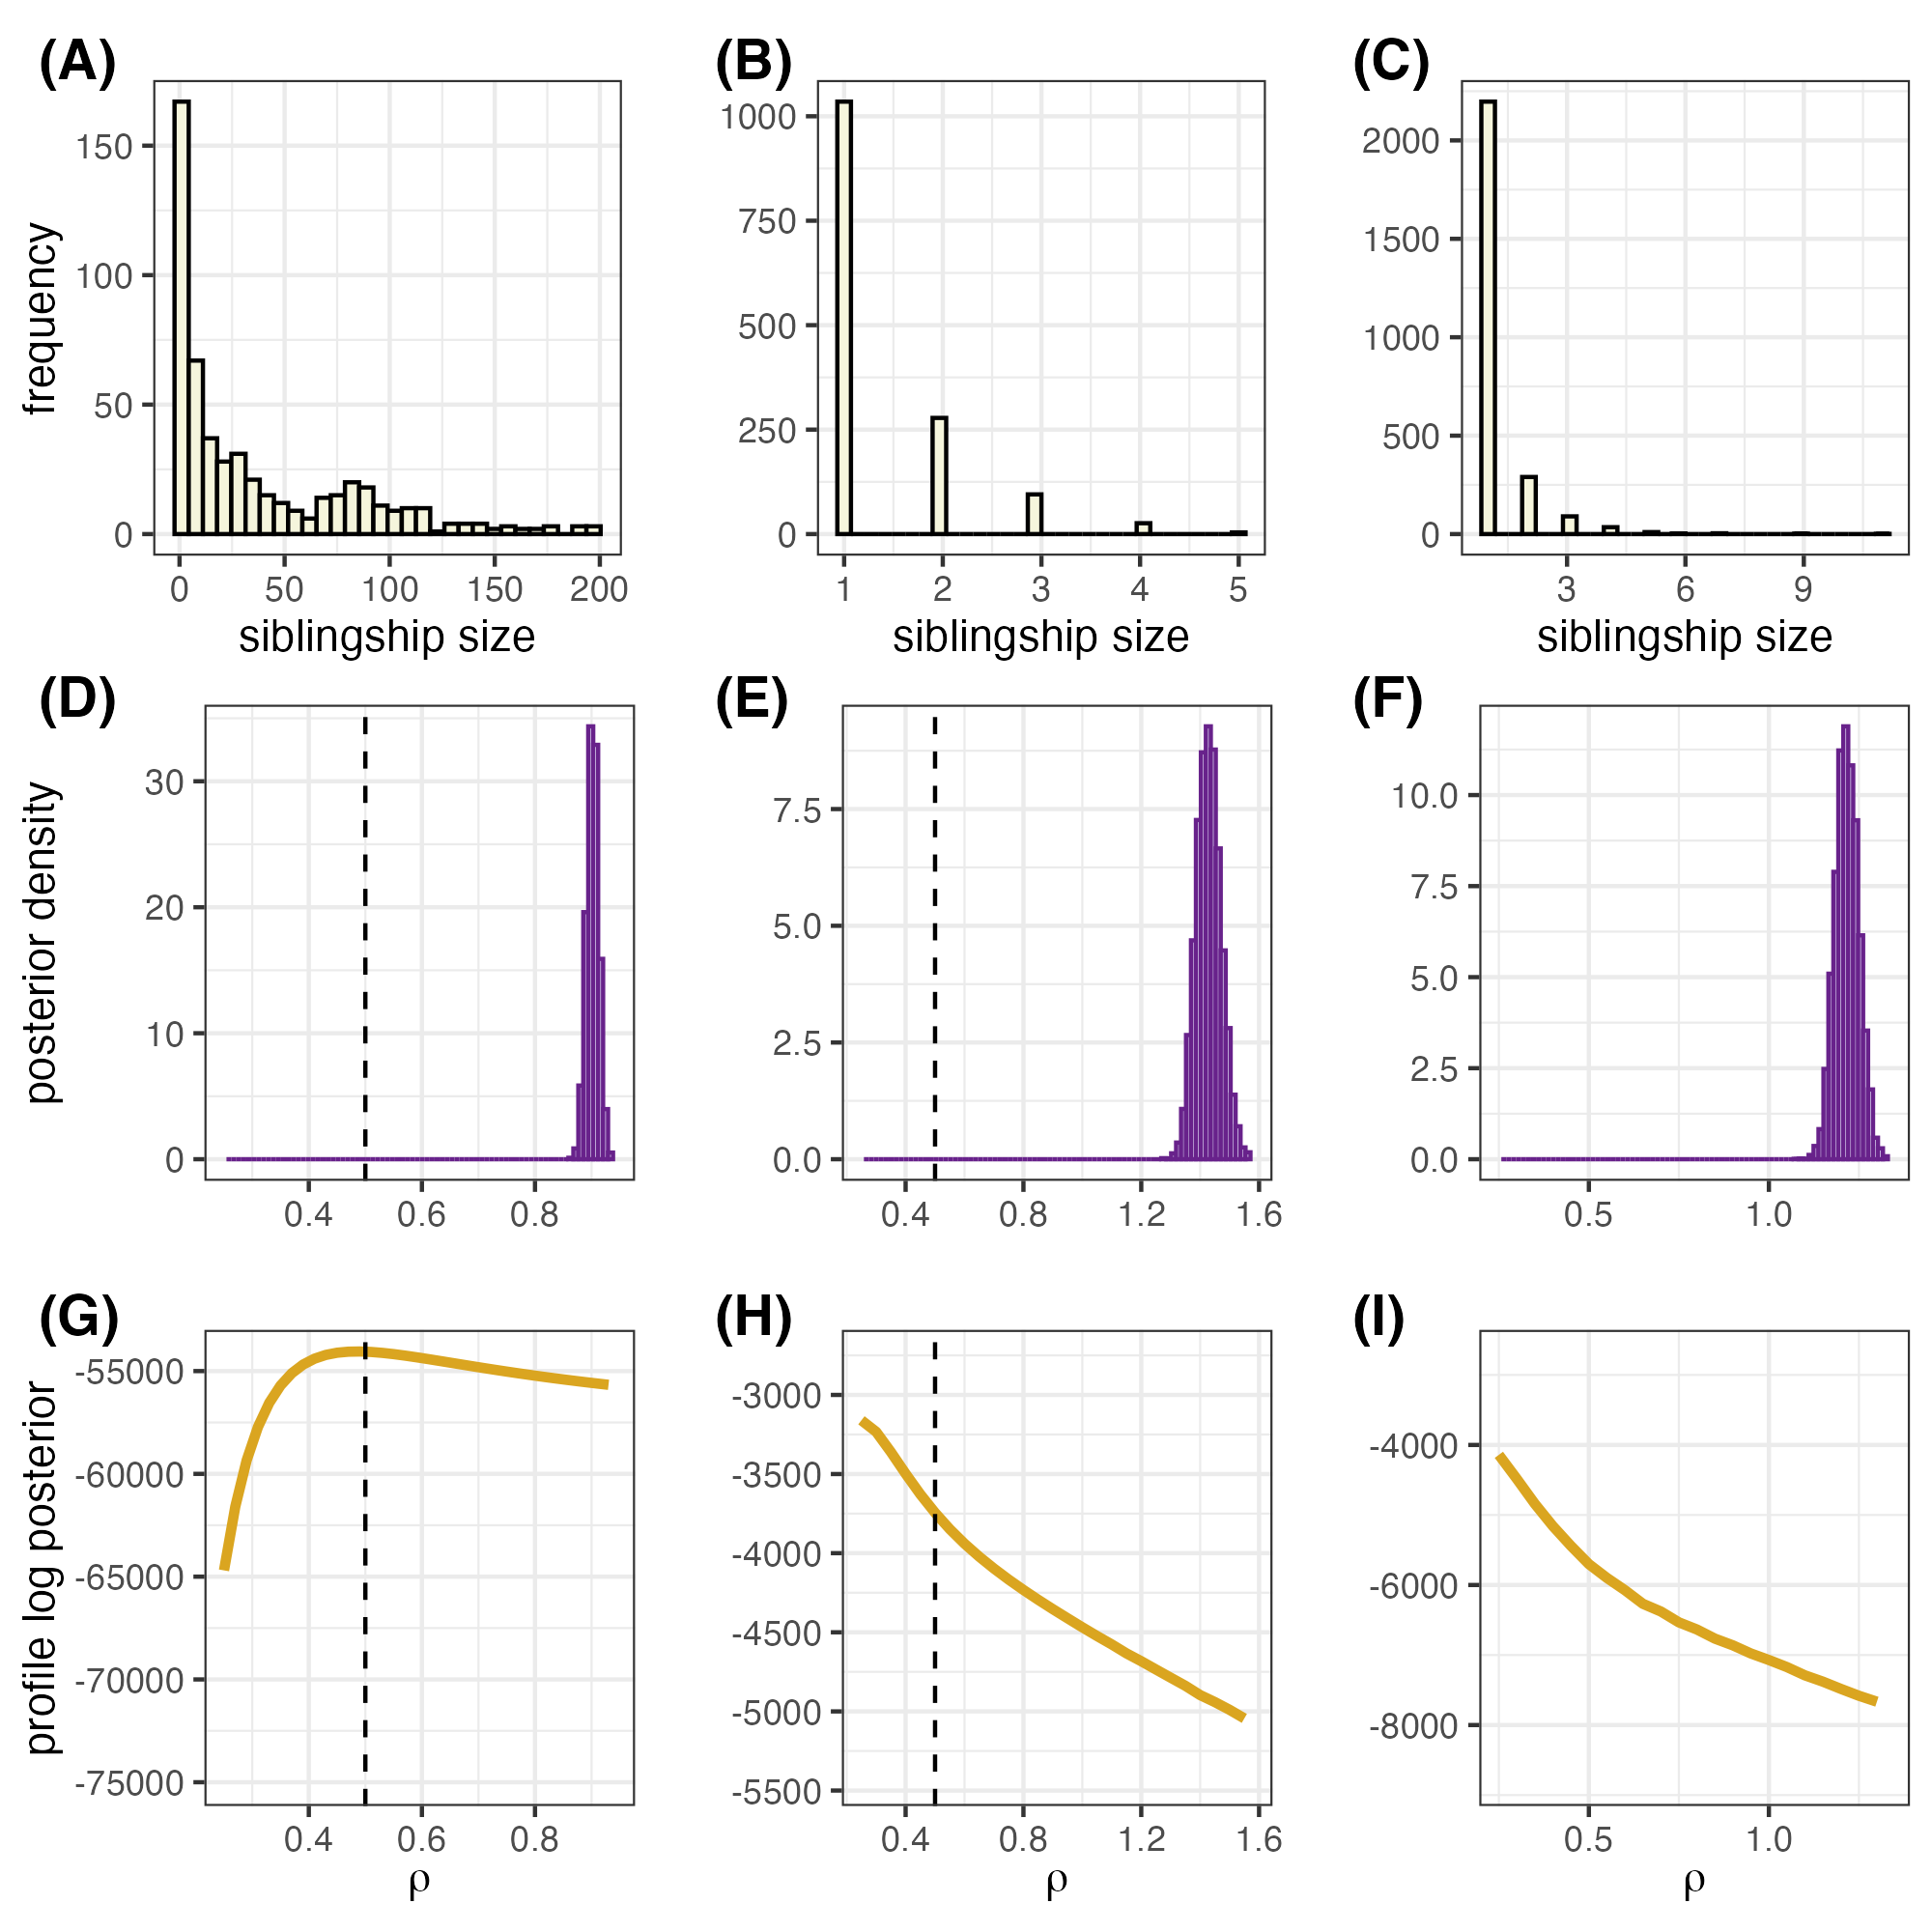
\includegraphics[width=\linewidth]{figures/fig1.png}
    \caption{Conditioning a simple foraging distance model on simulated and real bumblebee spatial mark-recapture datasets. We perform inference using the initial model described in the Methods, and three datasets: an ideal simulated dataset (A, D, G), with an average siblingship size of 37 individuals per colony, a biologically realistic simulated dataset (B, E, H) with an average siblingship size of 1.4 individuals, and an empirical dataset for \emph{B. impatiens} (C, F, I) with an average siblingship size of 1.3 individuals. Panels A-C show the distribution of siblingship sizes for each dataset; D-F show the posterior distributions of $\rho$, the foraging length scale; G-I show the optimal unnormalized log posterior for fixed values of $\rho$. The vertical dashed lines in D, E, G, and H represent the data-generating $\rho$ used for simulations.}
    \label{fig:fig1}
\end{figure}

\begin{figure}[H]
    \centering
    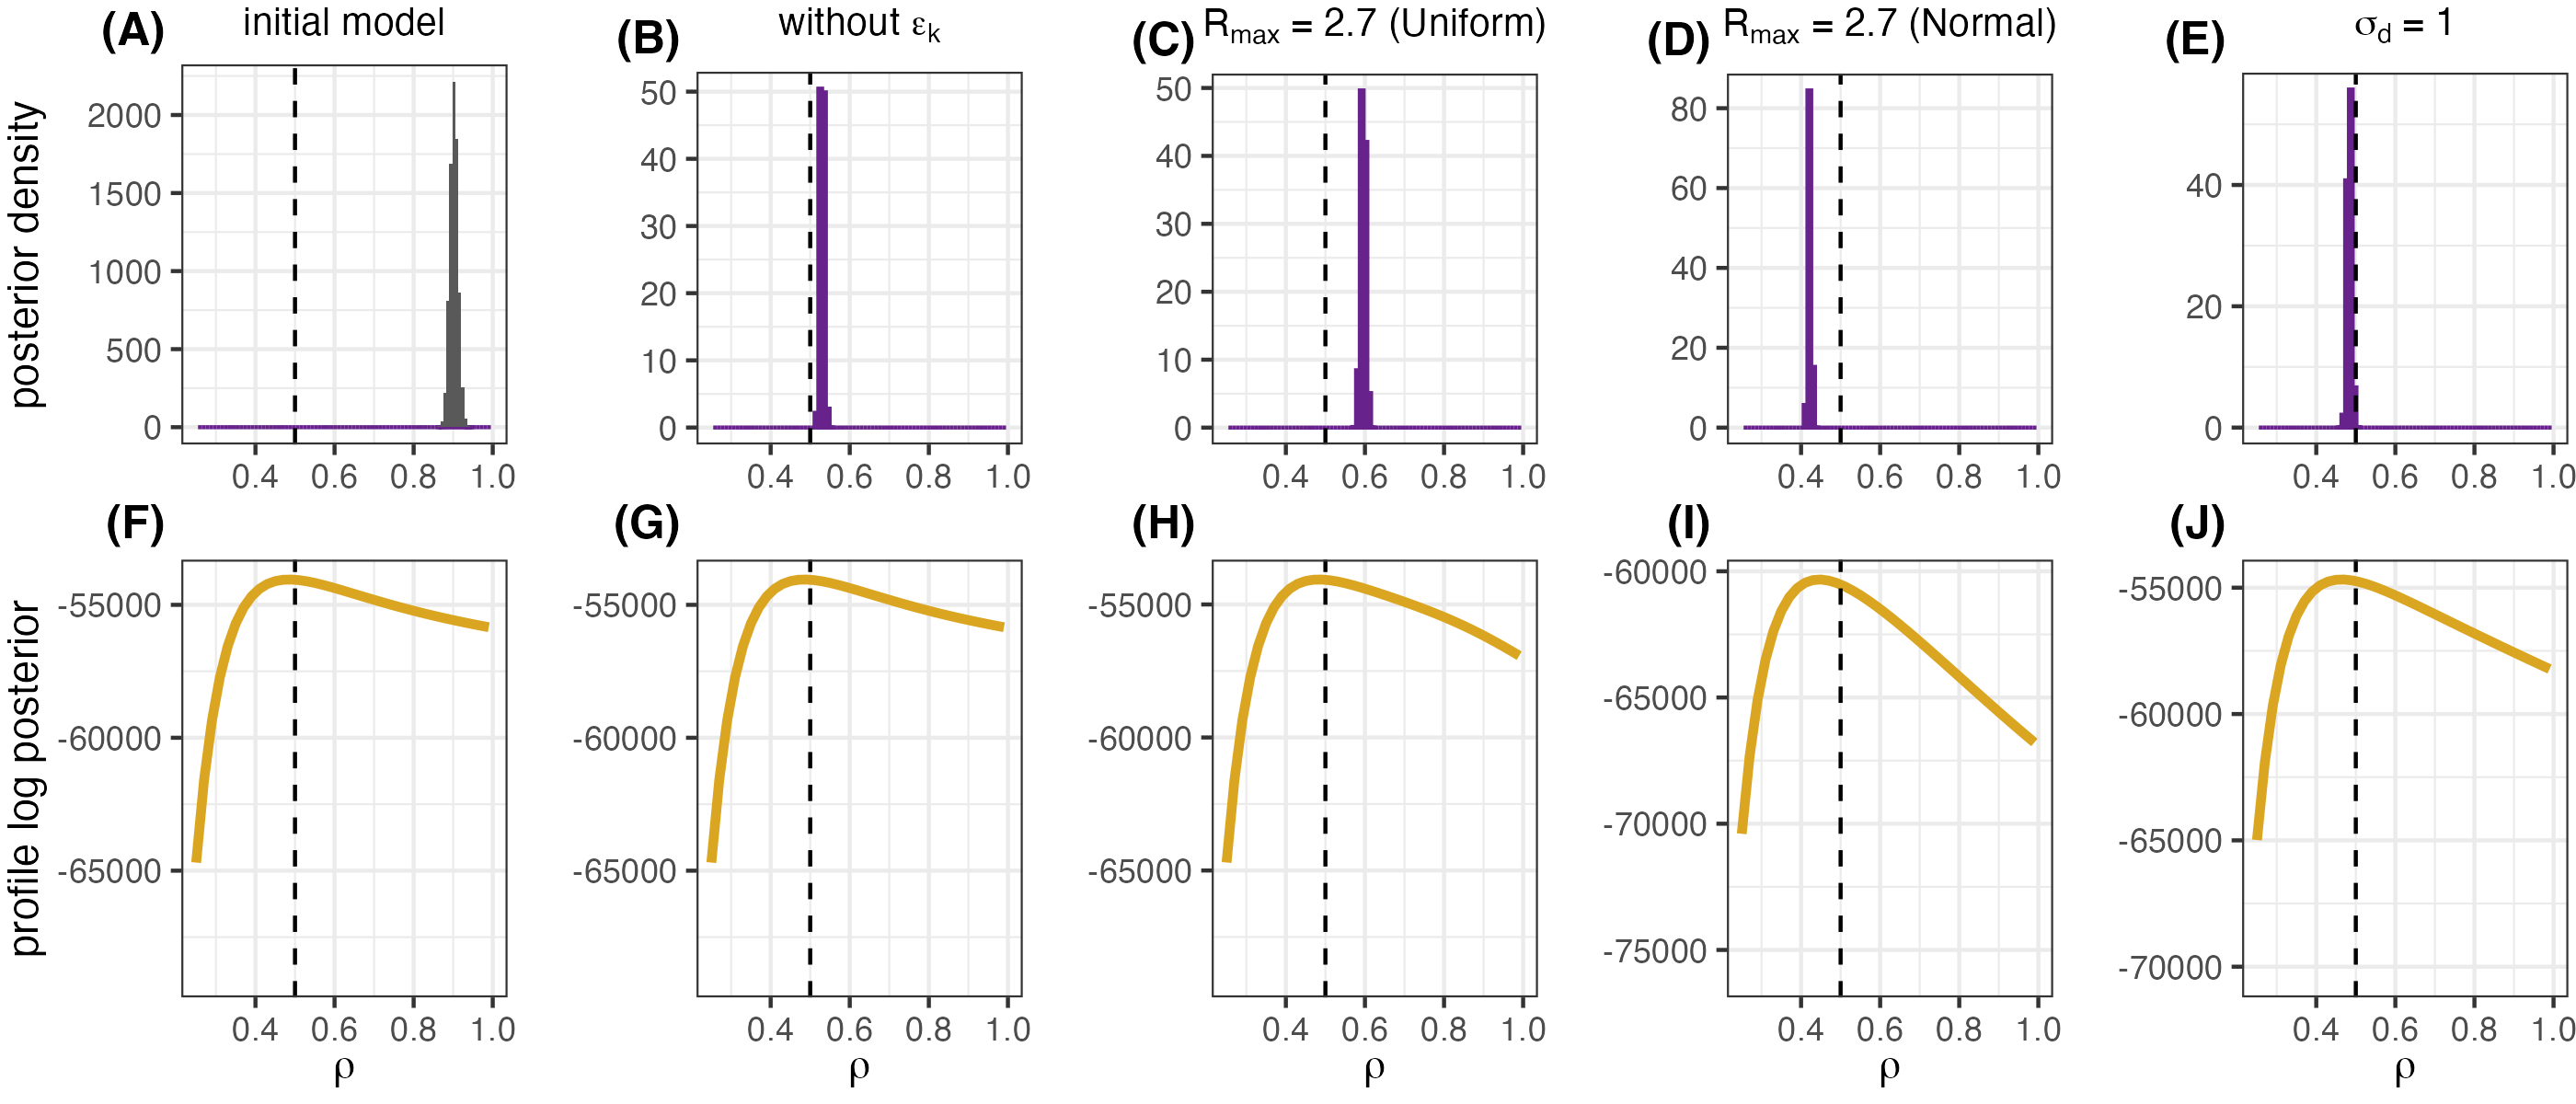
\includegraphics[width=\linewidth]{figures/perfectentropyfix.png}
    \vspace{-20pt}
    \caption{Exploring solutions for constraining high-dimensional $\delta$ using an ideal simulated dataset. Each column represents a different strategy for reducing the parameter space volume for $\delta$: A,F: initial model, B,G: initial model without trap-specific intercepts $\epsilon_k$, C,H: penalizing the likelihood with a pseudo-Uniform, D,I: penalizing the likelihood with a Gaussian, E,J: multivariate Gaussian prior on $\delta_i$. A-E) posterior density of $\rho$ inferred from the model; F-J) optimal unnormalized log posterior for fixed values of $\rho$. Vertical dashed lines denote data-generating $\rho$.}
    \label{fig:perfectentropyfix}
\end{figure}

\begin{figure}[H]
    \centering
    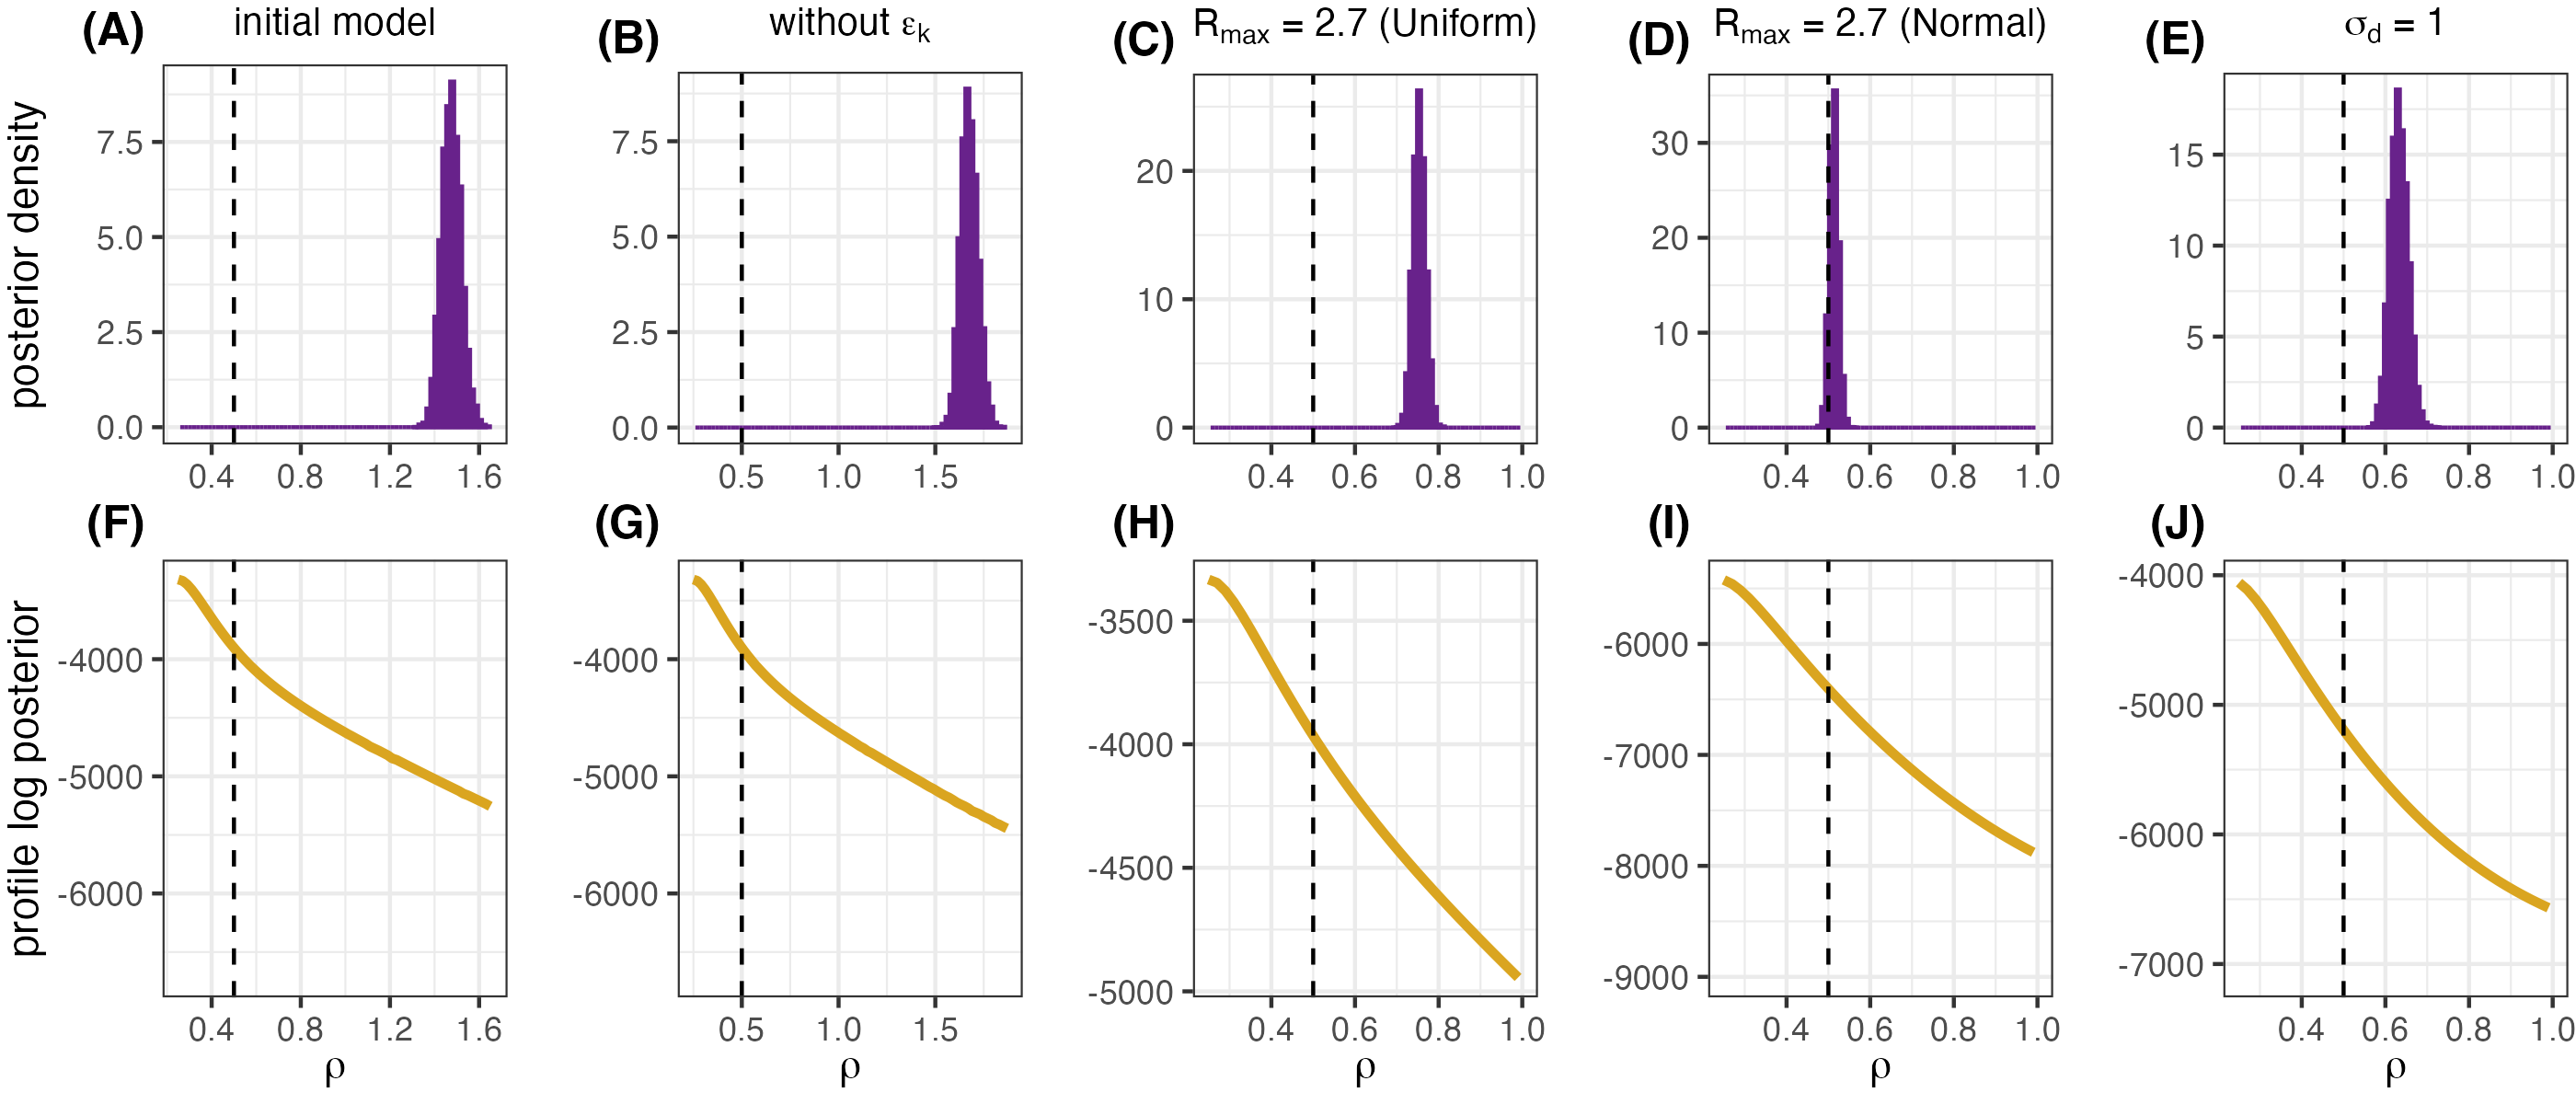
\includegraphics[width=\linewidth]{figures/realentropyfix.png}
    \vspace{-20pt}
    \caption{Exploring solutions for constraining high-dimensional $\delta$ using a biologically realistic simulated dataset. Each column represents a different strategy for reducing the parameter space volume for $\delta$: A,F: initial model, B,G: initial model without trap-specific intercepts $\epsilon_k$, C,H: penalizing the likelihood with a pseudo-Uniform, D,I: penalizing the likelihood with a Gaussian, E,J: multivariate Gaussian prior on $\delta_i$. A-E) posterior density of $\rho$ inferred from the model; F-J) optimal unnormalized log posterior for fixed values of $\rho$. Vertical dashed lines denote data-generating $\rho$.}
    \label{fig:realentropyfix}
\end{figure}

\begin{figure}[H]
    \centering
    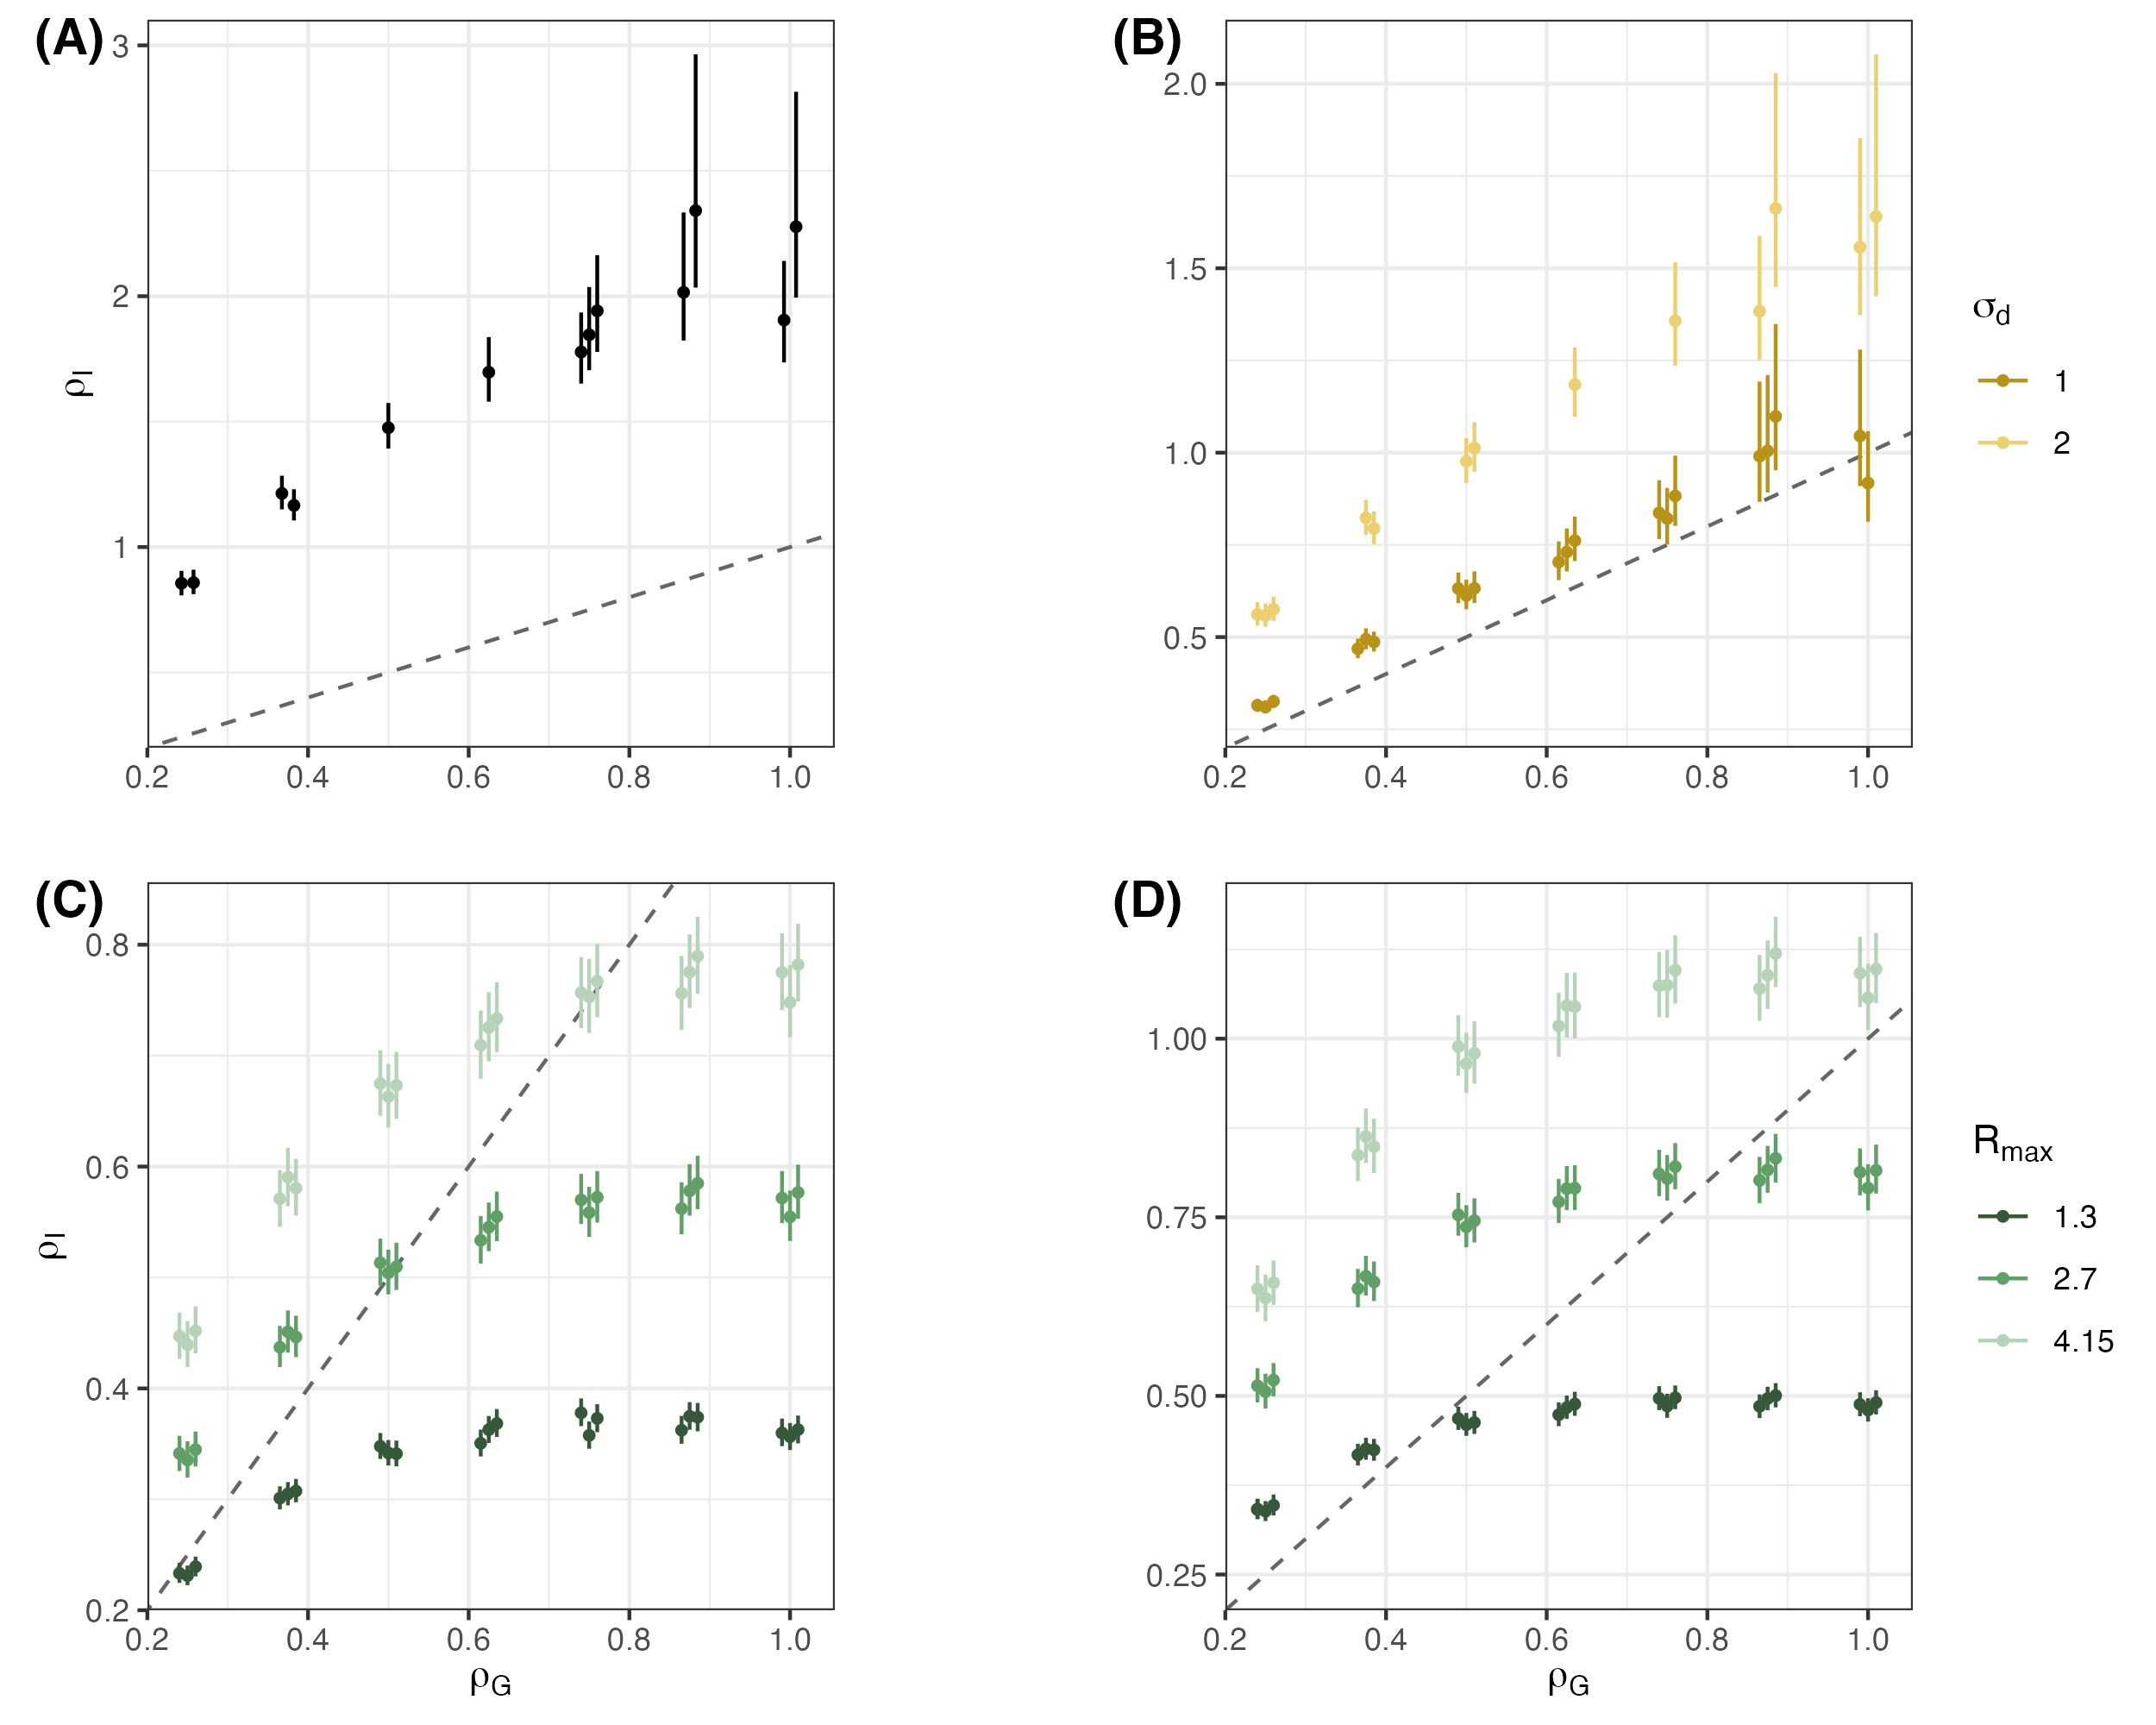
\includegraphics[width=\linewidth]{figures/simplesim.png}
    \vspace{-20pt}
    \caption{Performance of $\delta$ constraints across a range of data-generating $\rho_G$. A) No prior or constraint of $\delta$, B) Bivariate Gaussian prior with standard deviation $\sigma_d$ in each (x,y) dimension, C) Gaussian penalization applied to the likelihood, D) Pseudo-Uniform penalization applied to the likelihood. Dashed lines denote $\rho_I = \rho_G$.}
    \label{fig:simplesim}
\end{figure}

\begin{figure}[H]
    \centering
    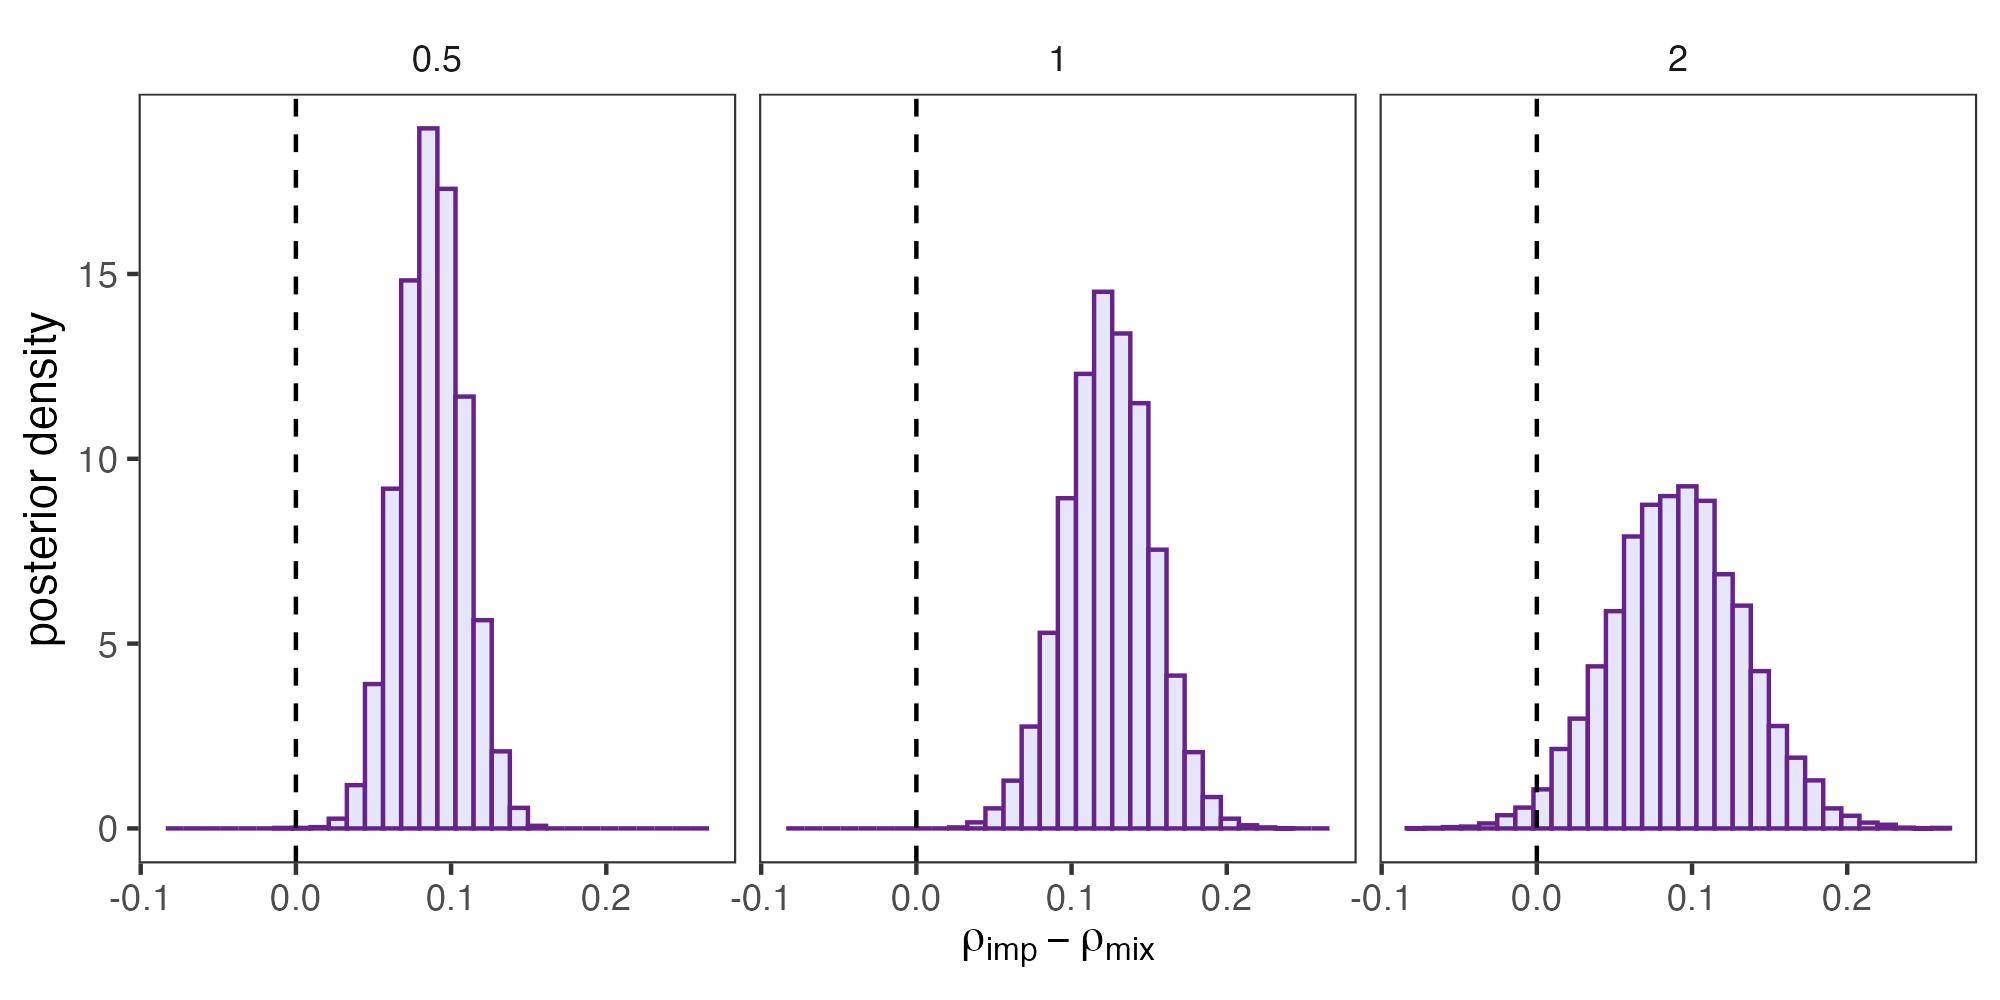
\includegraphics[width=\linewidth]{figures/impvsmix.png}
    \vspace{-20pt}
    \caption{Differences in the foraging scale $\rho$ for invasive \emph{B. impatiens} and native \emph{B. mixtus} are shown for models utilizing $\sigma_d = 0.5, 1, 2$ km. }
    \label{fig:impvsmix}
\end{figure}

\begin{figure}[H]
    \centering
    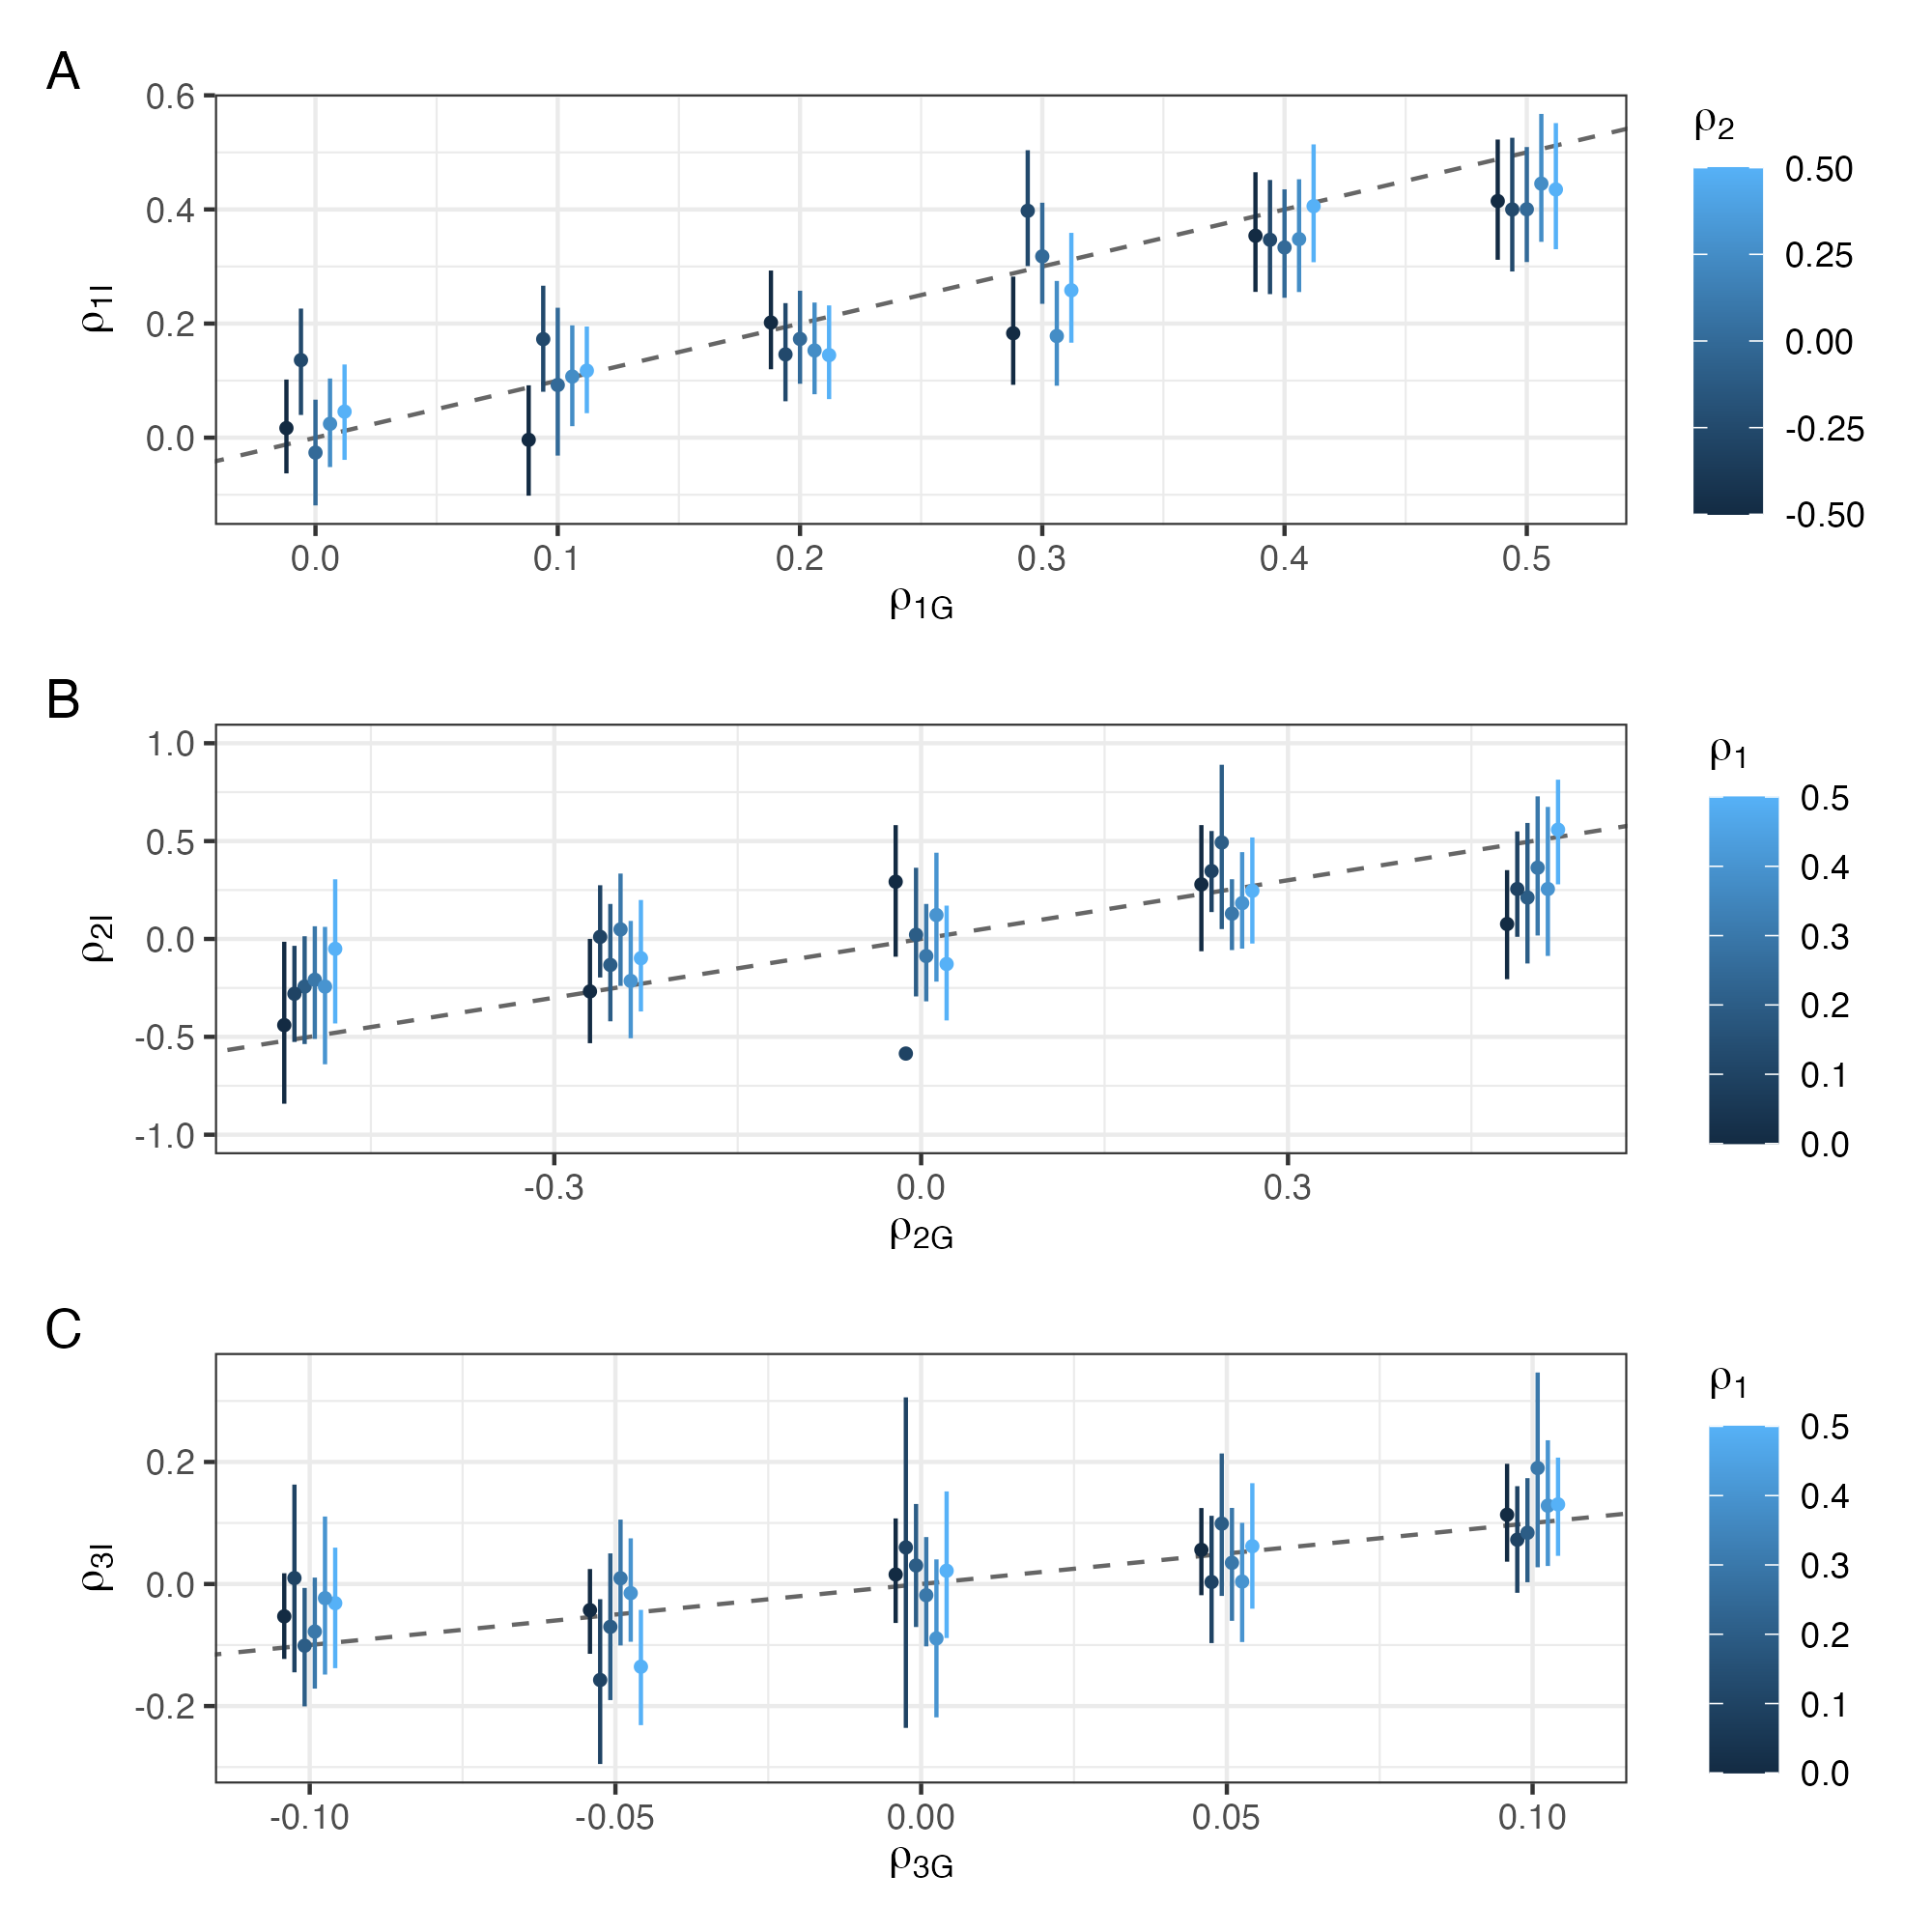
\includegraphics[width=\linewidth]{figures/interactions.png}
    \vspace{-20pt}
    \caption{Inference for a model incorporating the effects of local resource quality ($\rho_1$), the effects of landscape-scale resource quality ($\rho_2$) and their interaction ($\rho_3$) on foraging scale. A) Model inferred values of $\rho_{1I}$ versus data-generating $\rho_{1G}$, colored by data-generating $\rho_2$. $\rho_3$ = 0. B) Model inferred values of $\rho_{2I}$ versus data-generating $\rho_{2G}$, colored by data-generating $\rho_1$. $\rho_3$ = 0. C) Model inferred values of $\rho_{3I}$ versus data-generating $\rho_{3G}$, colored by data-generating $\rho_1$. $\rho_2$ = 0.}
    \label{fig:interactions}
\end{figure}

\clearpage
\printbibliography
\clearpage

\noindent \textbf{Appendix} \\

\noindent \textbf{Data Simulation} \\

\noindent Our method for simulating spatially explicit siblingships generally follows \textcite{pope_inferring_2017}. \\


We begin with six trapping grids with trap coordinates/configuration identical to our true study landscapes (described below). Colonies $i \in \mathbb{C}$ are simulated uniformly at random throughout the ``landscape" (more exactly, they are simulated uniformly at random within 2km of the trapping grids, as this reduces the computational load and speeds up simulation. For realistic simulation parameters, colonies beyond this distance are very rarely observed at traps).

We then sampled individuals from colonies $i \in \mathbb{C}$ captured at traps $k \in \mathbb{K}$ from the joint distribution $\Pr(s, c \mid s \in \kappa)$, where $\{s,c\}$ are the indices of a random visitation event of an individual from colony $c \in \mathbb{C}$ to grid cell $s \in \mathbb{J}$.

To do this, we first sampled a trap ($k$) from

\[
\Pr(s = k \mid s \in \kappa) \;=\; \frac{\Pr(s = k)}{\Pr(s \in \kappa)} \tag{1}
\]

where

\[
\Pr(s = k) \;=\; \sum_{i \in C} \Pr(s = k \mid c = i)\,\Pr(c = i)
\]

and

\begin{align*}
\Pr(s \in \kappa) 
    &= \sum_{i \in \mathbb{C}} \Pr(s \in \kappa \mid c = i)\,\Pr(c = i) \\[0.5em]
    &= \sum_{i \in \mathbb{C}} \sum_{k \in \kappa} \Pr(s = k \mid c = i)\,\Pr(c = i)
\end{align*}


Combining these statements gives a probability of sampling from trap $k$ of:

\[
\Pr(s = k \mid s \in \kappa) \;=\; \frac{\sum_{i \in C} \Pr(s = k \mid c = i)\,\Pr(c = i)}{\sum_{i \in \mathbb{C}} \sum_{k \in \kappa} \Pr(s = k \mid c = i)\,\Pr(c = i)} \tag{2}
\]

We then sampled a colony ($i$) from

\begin{align*}
\Pr(c = i \mid s = k)
  &= \frac{\Pr(s = k \mid c = i) \Pr(c = i)}{\Pr(s = k)} \\[0.5em]
  &= \frac{\Pr(s = k \mid c = i) \Pr(c = i)}{\sum_{i \in \mathbb{C}} \Pr(s = k \mid c = i)\,\Pr(c = i)} \tag{3}
\end{align*}


We define the foraging kernel of workers from colony $i$ as

\[
\Pr(s = k \mid c = i)
\;=\; 
\frac{\lambda_i(k)}{\sum_{j \in J} \lambda_i(j)} \tag{4}
\]

where the visitation intensity of individuals from colony $i$ to location $j$ is 

\[
log(\lambda_i(j)) = -\frac{1}{2}\left(\frac{\lVert x_j - \delta_i \rVert}{\rho}\right)^2 \tag{5}
\]


$x_j$ are the spatial coordinates of any grid cell in the raster, and $\delta_i$ are the spatial coordinates of colony $i$. The foraging kernel in this example is therefore symmetrical and exponentially decaying as a function of distance from the colony location. This means that the total visitation rate of each colony across the landscape ($\sum_{j \in J} \lambda_i(j)$) is the same for all colonies, and can be represented using the constant $\mathbb{D}$. $\Pr(c = i)$ is the proportion of all bees in the landscape originating from colony $i$, e.g., $\Pr(c = i) = \frac{n_i}{N}$ where $n_i$ is the number of bees from colony $i$, and $N = \sum_{i \in \mathbb{C}} n_i$ is the total number of bees in the landscape.

Combining (4) with (2) and (3) gives the probability of sampling an individual from trap $k$

\[
\Pr(s = k \mid s \in \kappa) \;=\; \frac{\sum_{i \in \mathbb{C}} \lambda_i(k) \frac{n_i}{N}}{\sum_{k \in \kappa} \sum_{i \in \mathbb{C}} \lambda_i(k) \frac{n_i}{N}}
\]

and the probability that the individual originates from colony $i$

\[
\Pr(c = i \mid s = k) \;=\; \frac{\lambda_i(k) \frac{n_i}{N}}{\sum_{i \in \mathbb{C}} \lambda_i(k) \frac{n_i}{N}}
\]

For each simulation, samples are drawn from $\Pr(s, c \mid s \in \kappa)$ until a stopping point (desired number of samples) is reached. $n_i$ is updated after each ``sampling event" to prevent oversampling from colonies located very close to traps.

To verify that the size of sampled siblingships (e.g., number of siblings per sibling group) accurately mirrors the distribution of siblingship sizes in real data, we compared our simulated distributions to the distribution of siblingshp sizes in our real data (Fig. \ref{fig:fig1} A-C).
%%%NOTE: make this into a proper comparison!!
We found that moderating the background density of colonies (i.e., the total number of colonies simulated on the landscape) was the most effective strategy for controlling average siblingship size. A higher background density of simulated colonies results in a higher proportion of singleton colonies (colonies represented by only a single individual). \\



\noindent \textbf{Data Collection} \\

\noindent \textbf{Study system} \\
Our study took place in the Lower Fraser Valley in southwestern British Columbia, Canada, in an agricultural system dominated by mixed vegetable, hay, and perennial berry production. Field surveys were conducted across six replicate landscapes (trapping grids). Each landscape encompassed roughly 3 sq km of farmland interspersed with rural/suburban residence. Landscapes were initially chosen to span a gradient of configurational and composition diversity metrics, including Shannon's diversity, edge density, and the ratio of annual to perennial crop cultivation. \\

\noindent \textbf{\textit{Bombus} collections and floral surveys} \\
Each landscape was surveyed during 10 sampling rounds in 2022 (May-August) and 17 sampling rounds in 2023 (March-August). We initially established thirty sampling transects (50 meters x 2 meters) in each landscape, spaced as evenly as possible based on land-access and the availability of foraging resources on which to observe bees. Transect turnover occurred within and between years due to changes in land access. However, the number of surveys per landscape per sampling round remained consistent (28.1 $\pm$ 1.9 (mean $\pm$ SD) in 2022, 30.2 $\pm$ 0.9 in 2023). When applicable, we incorporate offset variables into our models to account for differences in survey effort per transect. A total of 289 transects (28,900$m^2$) were visited over the course of study.

\textit{Bombus} surveys at each transect entailed 5 minutes of active search time (totaling 140 hours in 2022 and 255 hours in 2023), during which the stopwatch was paused whenever a foraging bumble bee was sighted. Specimens were captured by netting, placed into sterile 15 mL tubes, and immediately placed on ice before transfer to a -80$^\circ$ C freezer at the end of the day.  Surveys were conducted on days when the temperature was above 12$^\circ$  C (10$^\circ$  C for queen surveys) and wind speeds below 2.5 m/s. In 2022, all \textit{Bombus} species were collected; in 2023 only the focal species (\textit{B. mixtus} and \textit{B. impatiens} were collected.

We identified all flowering plants within each 50 m x 2 m transect to species or genus using the iNaturalist Seek mobile application. Seek applies an internal confidence threshold for species-level identifications; in a validation study of 857 professionally identified plant images, it produced no false species-level identifications above this threshold, and flower presence significantly improved genus-level accuracy \parencite{hart_assessing_2023}. We classified plants to species when the confidence threshold was exceeded---which occurred in most cases---or to genus when it was not, with rare instances achieving only family-level identification. Inflorescence abundance was visually estimated in the field for each species along each transect. Estimates were assigned to one of five log-scale abundance categories (0-4: 0 = 1-10, 1 = 11-100, 2 = 101=1,000, 3 = 1,001-10,000, 4 = $\geq 10,000$). We selected these categories to reflect the floral abundances that bumblebees were likely to encounter and respond to in our study landscapes, which included both rare resources (< 10) and highly abundant resources such as mass-flowering crops and flowering trees. Floral surveys were later filtered to exclude species that bumble bees were never observed visiting. This filtering step was included to reduce the noise introduced by several herbaceous weeds with flowers too small to attract or support bumble bee foragers that were frequently observed on the transects in high abundance. \\

\noindent \textbf{PCR Amplification and Fragment Analysis} \\
DNA was extracted from the mid-leg basitarsus and tarsus (distal tarsus only for queens) using the HOTSHOT protocol \parencite{truett_preparation_2000}. Specimens were microsatellite genotyped at loci BT10, BTERN01, BL13, BL15, B126, BTMS0057, BTMS0059, BTMS0062, BTMS0083 (both species), BTMS0066, BTMS0086, BTMS0104, BTMS0126, BTMS0136 (\textit{B. mixtus} only), BT28, BT30, B10, B96, B124, BTMS0073, and BTMS0081 (\textit{B. impatiens} only) \parencite{estoup_monoandry_1995, estoup_genetic_1996, reber_funk_microsatellite_2006,stolle_novel_2009}. One primer for each locus was individually dye-labelled using 6FAM, NED, PET, or VIC, and loci were amplified in two multiplex reactions per individual. Each multiplex reaction contained 4$\mu$L of template DNA, 1$\mu$L of 10X primer mix, and 5$\mu$L of Qiagen 2X Multiplex PCR Master Mix (Qiagen, Hilden, Germany). Diluted PCR products were submitted for automated fragment sizing at the UBC Sequencing and Bioinformatics Consortium (\textit{B. mixtus}) and the Utah State Center for Integrated Biosystems (\textit{B. impatiens}). 1$\mu$L of each sample was added to 8.85$\mu$L of Hi-Di formamide and 0.15$\mu$L of LIZ500 size standard; \textit{B. mixtus} fragments were analyzed on an Applied Biosystems 3730XL 96-capillary DNA Analyzer and \textit{B. impatiens} fragments were analyzed on an Applied Biosystems 3730 DNA Analyzer (Applied Biosystems, Foster City, CA, USA). Microsatellite peaks were assigned manually using the software Geneious Prime 2024.0.5 (https://www.geneious.com). Scoring error rates were assessed by re-genotyping a panel of 96 individuals per species, and loci with observed error rates $\geq$3\% were discarded from further analyses (BL15 for both species). \\

\noindent \textbf{Colony Assignments} \\
We used an iterative approach to assign workers and queens to their natal colonies. First, using the pedigree reconstruction software COLONY2.0.6.5 \parencite{jones_colony_2010} (hereafter, COLONY), we assigned full siblingships based on all available microsatellite data, assuming male and female monogamy and no inbreeding. A single run was carried out for each species and year, using the software's full-likelihood approach and no siblingship size scaling or priors. Sibling pairs were maintained when $P_{fullsib dyad} = 1$. A single individual from each putative colony (including non-circular colonies, described below) was maintained for downstream analyses of locus quality.

While COLONY can account for inbreeding at the population level, locus-specific estimates of $F_{is}$ should generally be similar to one another for a given population, reflecting their shared evolutionary history. Loci with $F_{is}$ estimates that deviate significantly from the species mean (across loci) may suffer from null alleles or other types of scoring errors that can bias siblingship assignment. We therefore tested individual locus deviations from population mean $F_{is}$ as a criterion for marker inclusion/exclusion. Single locus $F_{is}$ estimates were computed for all site, year, species groups following \parencite{weir_estimating_1984} in the package \emph{genepop} \parencite{rousset_genepop007_2008}. We then fit linear models to $F_{is}$ estimates with locus and site as fixed predictors. We used sum-to-zero coding so that model intercepts represented mean $F_{is}$ across all loci, and calculated the estimated marginal mean of each locus using the \emph{emmeans} package \parencite{lenth_emmeans_2024}. We iteratively removed loci with $F_{is}$ significantly different from the species mean $F_{is}$, starting with the locus with the greatest deviation, and re-running the model after each removal. We did not apply an adjustment for multiple-hypothesis testing, but instead utilized a relatively stringent p-value ($\alpha$ = 0.01) for removal of loci. This process resulted in the removal of loci BTERN01, BTMS0104, and BTMS0059 from downstream analyses for \emph{B. mixtus} and removal of BTMS0073 and BT28 for \emph{B. impatiens}.

Next, we checked locus pairs for linkage disequilibrium (LD). Marker linkage can lead to non-independent assortment, a condition which violates the assumptions of most parentage reconstruction software and can result in overconfidence in estimated sibling pairs. LD was calculated for each locus pair in each population (site, year, species groups) in \emph{genepop}. We applied a Bonferroni correction for multiple hypothesis testing, and flagged locus pairs which showed significant deviations in $>2$ populations. For \emph:{B. mixtus}, four locus pairs showed signs of LD, but each occurred at only a single site in a single year, so we chose to maintain all loci. For \emph{B. impatiens}, there was strong evidence for linkage disequilibrium between BTMS0057 and BL13 (7 out of 12 populations showed significant LD following Bonferroni correction). To determine which locus to maintain, we calculated the polymorphic information content (PIC) using the package \emph{PopGenUtils} \parencite{tourvas_popgenutils_2025}. We found that BTMS0057 had higher PIC in both years (PIC = 0.78) compared to BL13 (PIC = 0.47 in 2022 and 0.45 in 2023). We therefore maintained BTMS0057 and removed BL13 from further analyses for \emph{B. impatiens}.

After locus quality screening, we calculated global and pairwise $F_{st}$ following \parencite{nei_molecular_1987} in the package \emph{hierfstat} \parencite{goudet_hierfstat_2005}. For both species and years, estimates of global $F_{st}$ were less than 0.005. Pairwise $F_{st}$ ranged from -0.002 to 0.01, indicating little or no genetic differentiation between surveyed sub-populations. Finally, we computed the marginal mean $F_{is}$ for each site to determine whether there was evidence for inbreeding following locus removal, and whether it varied between sites.
Because we found evidence for only minor inbreeding (e.g., $F_{is} < 0.05$) we ran all final colony assignments using the no-inbreeding model. Given the very low estimates of global and pairwise $F_{st}$, we chose to combine sites for siblingship assignments to maximize the accuracy of allele frequency estimation.

We performed final colony assignments using separate COLONY runs for each species-year combination. To determine optimal software settings, we tested COLONY performance on simulated datasets using allele frequencies derived from our true data (data not shown). Colony assignments were performed using a single COLONY run for each species-year combination. We used exclusion tables to prevent the assignment of siblingships between individuals originating from different replicate landscapes. Each run assumed male and female monogamy and no inbreeding, and utilized no prior on siblingship size and no siblingship size scaling. All runs were performed using the Linux command line version of the software, with run length set to "long", likelihood set to "full-likelihood" and precision set to "high precision." Sibling pairs were maintained with $P_{fullsib dyad} \geq 0.995$. Because we used full sibling dyad probabilities rather than sibling cluster probabilities to perform assignments, we resolved non-circular families (e.g., individual A related to individual B, B related to C, but A \emph{not} related to C) manually (heuristic described elsewhere, if you've read this far, Charles, I'm deeply impressed). Overall, the results of our simulation suggest that previous studies of fine-scale lineage in bumblebees using similar genetic datasets may suffer from high false positive rates due to insufficiently stringent probability thresholds for siblingship assignment.
\clearpage

\renewcommand{\thefigure}{A\arabic{figure}}
\setcounter{figure}{0}
\begin{figure}[H]
    \centering
    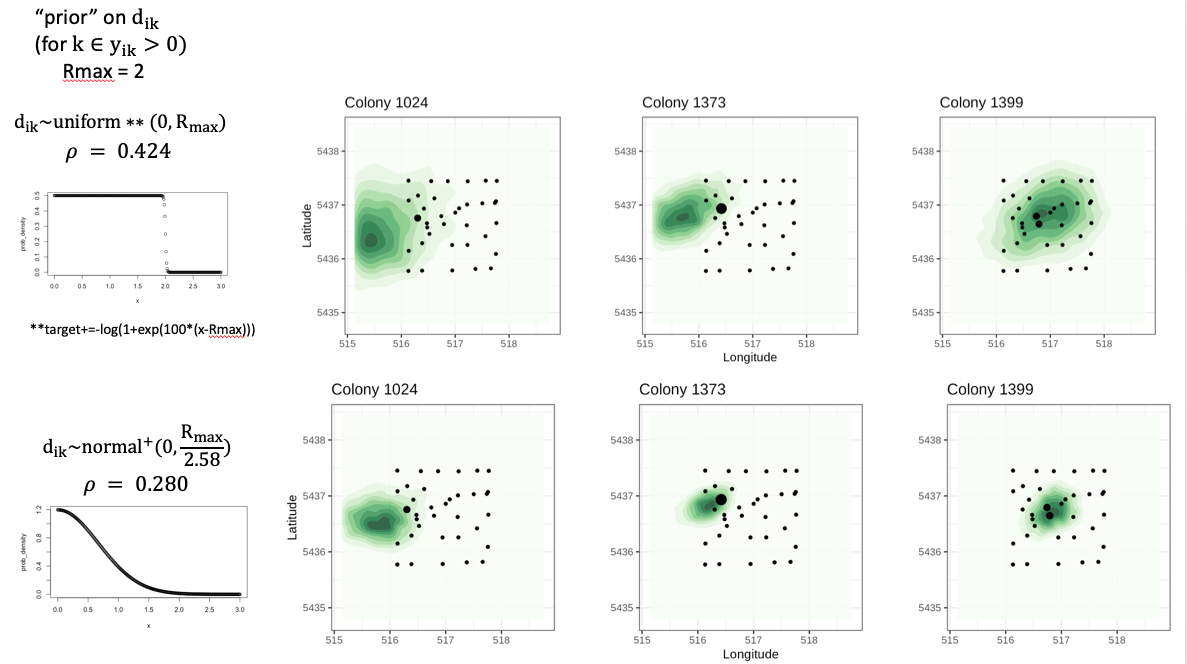
\includegraphics[width=\linewidth]{figures/appendix1.png}
    \vspace{-20pt}
    \caption{Penalizations applied to the likelihood when the distance from $\delta_i$ to the trap(s) where colony $i$ is observed ($d_{ik}$) is greater than $R_{max}$. Estimated colony locations ($\delta_i$) are illustrated for three colonies of \emph{B. impatiens}.}
    \label{fig:A1}
\end{figure}

\end{document}
